\documentclass[a4paper,12pt]{article}

\usepackage[english]{babel}
\usepackage{graphicx}

\begin{document}

\begin{table}[h!]
  \begin{center}
    \begin{tabular}{| c | c |}
    \hline
    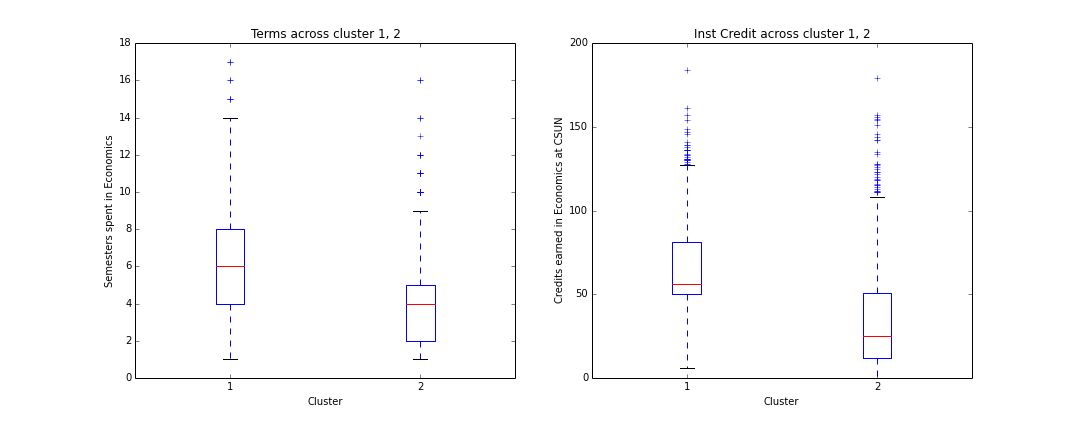
\includegraphics[width=0.5\textwidth]{figures/box-Economics}
    &
    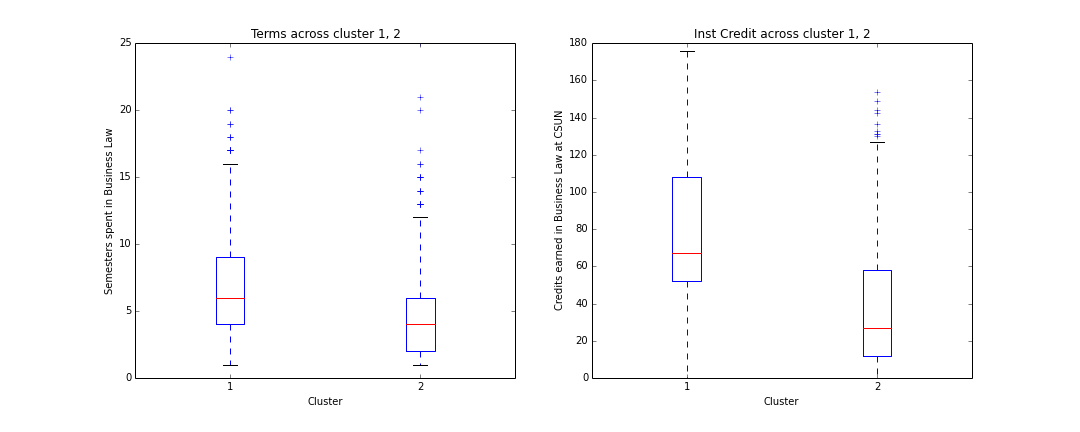
\includegraphics[width=0.5\textwidth]{figures/box-Business-Law}
    \\
    \hline
    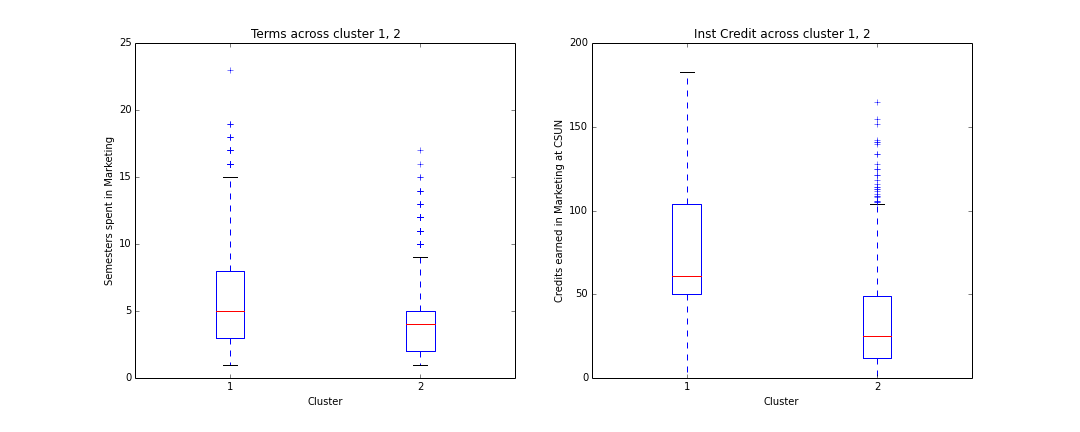
\includegraphics[width=0.5\textwidth]{figures/box-Marketing}
	&    
    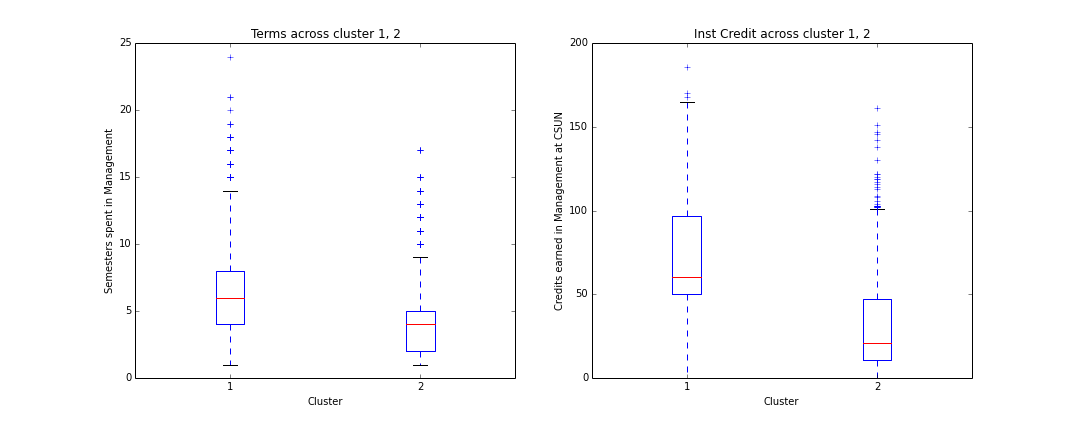
\includegraphics[width=0.5\textwidth]{figures/box-Management}
    \\
    \hline
    \end{tabular}
  \end{center}
  \caption{A simple table}
\end{table}


Notice how the tables and figures
have independent counters.

\end{document}